\documentclass[tikz]{standalone}
\usepackage{amsmath, amssymb}
\usetikzlibrary{arrows.meta, positioning, shapes.geometric}

\begin{document}
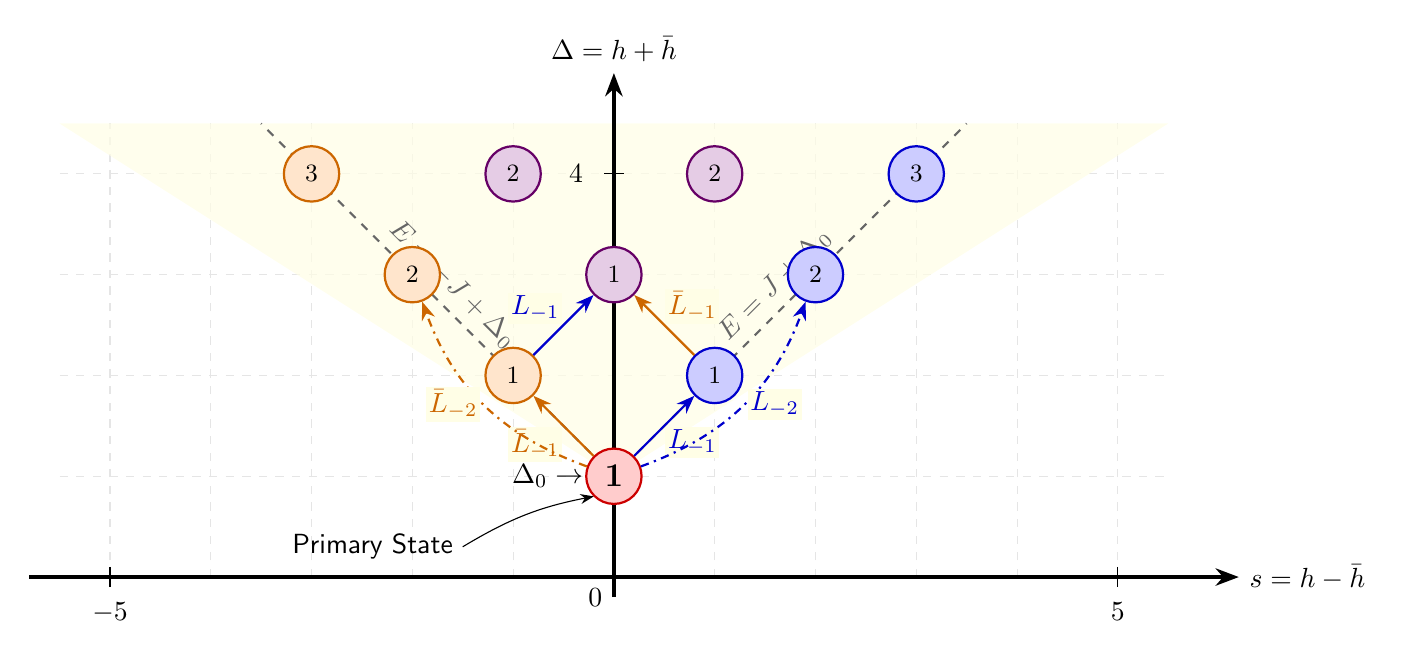
\begin{tikzpicture}[x=1.6cm, y=1.6cm, >=Stealth, font=\sffamily,scale=.8]

    % ==========================================
    % 1. BACKGROUND GRID & CONE
    % ==========================================
    % Grid
    \draw[step=1.0, gray!20, thin, dashed] (-5.5, 0) grid (5.5, 4.5);
    
    % Cone Fill
    \fill[yellow!10, opacity=0.7] (0,1) -- (5.5, 4.5) -- (-5.5, 4.5) -- cycle;
    
    % Cone Boundaries (Unitarity-like bounds for this module)
    \draw[thick, dashed, black!60] (0,1) -- (3.5, 4.5) node[midway, sloped, above] {$E = J + \Delta_0$};
    \draw[thick, dashed, black!60] (0,1) -- (-3.5, 4.5) node[midway, sloped, above] {$E = -J + \Delta_0$};

    % ==========================================
    % 2. AXES
    % ==========================================
    % X-axis : Angular momentum
    \draw[->, line width=1.2pt] (-5.8, 0) -- (6.2, 0) node[right, align=center] {$s = h - \bar{h}$};
    
    % Y-axis : Energy / Scaling Dimension
    \draw[->, line width=1.2pt] (0, -0.2) -- (0, 5) node[above, align=center] {$\Delta = h + \bar{h}$};

    % Axis Tick Marks
    \draw (5, 0.1) -- (5, -0.1) node[below=2pt] {$5$};
    \draw (-5, 0.1) -- (-5, -0.1) node[below=2pt] {$-5$};
    \node[below left=1pt] at (0,0) {$0$};
    \draw (0.1, 4) -- (-0.1, 4) node[left=4pt] {$4$};
    \draw (0.1, 1) -- (-0.1, 1) node[left=4pt] {$\Delta_0 \to$}; % Mark the base energy level

    % Title
    %\node[font=\Large\bfseries] at (0, 7.8) {Conformal Tower (Verma Module) of a Primary State};
    
    % ==========================================
    % 3. GENERATE NODES (LATTICE OF DESCENDANTS)
    % ==========================================
    
    \foreach \na in {0,...,3}{
        \foreach \nb in {0,...,3}{
            
            % Check condition na + nb <= 3
            \pgfmathtruncatemacro{\sumN}{\na + \nb}
            \ifnum\sumN<4
                
                % Compute Spin (J) and Energy (E) coordinates
                \pgfmathtruncatemacro{\J}{\na - \nb}
                \pgfmathtruncatemacro{\EE}{1 + \na + \nb}
                
                % Safely calculate degeneracy using inline arrays instead of \ifcase
                % P(n) for n=0..5 -> 1, 1, 2, 3, 5, 7
                \pgfmathtruncatemacro{\partN}{{1,1,2,3,5,7}[\na]}
                \pgfmathtruncatemacro{\partNb}{{1,1,2,3,5,7}[\nb]}
                \pgfmathtruncatemacro{\mult}{\partN * \partNb} % Combines multiplicies
                
                % Default node style (Mixed)
                \def\nodecol{violet!80!black}
                \def\fillcol{violet!20}
                \def\styletxt{\small}
                
                % Pure anti-holomorphic chain (\na = 0)
                \ifnum\na=0
                    \def\nodecol{orange!80!black}
                    \def\fillcol{orange!20}
                \fi
                
                % Pure holomorphic chain (\nb = 0)
                \ifnum\nb=0
                    \def\nodecol{blue!80!black}
                    \def\fillcol{blue!20}
                \fi
                
                % Set Primary State specifically (both 0)
                \ifnum\sumN=0
                    \def\nodecol{red!80!black}
                    \def\fillcol{red!20}
                    \def\styletxt{\bfseries\large}
                \fi

                % Draw the Node uniquely named (N_\na_\nb)
                \node[
                    draw=\nodecol, 
                    fill=\fillcol, 
                    circle, 
                    thick, 
                    inner sep=0pt, 
                    minimum size=20pt, 
                    text=black, 
                    font=\styletxt
                ] (N_\na_\nb) at (\J, \EE) {\mult};
                
            \fi
        }
    }

    % ==========================================
    % 4. VIRASORO ACTION ARROWS (DYNAMICS)
    % ==========================================
    % L_{-1} actions (Move Right + Up)
    \draw[-Stealth, thick, blue!80!black] (N_0_0) -- (N_1_0) 
        node[midway, below right, fill=yellow!10, inner sep=1pt] {$L_{-1}$};
        
    \draw[-Stealth, thick, blue!80!black] (N_0_1) -- (N_1_1) 
        node[midway, above left, fill=yellow!10, inner sep=1pt] {$L_{-1}$};

    % \bar{L}_{-1} actions (Move Left + Up)
    \draw[-Stealth, thick, orange!80!black] (N_0_0) -- (N_0_1) 
        node[midway, below left, fill=yellow!10, inner sep=1pt] {$\bar{L}_{-1}$};
        
    \draw[-Stealth, thick, orange!80!black] (N_1_0) -- (N_1_1) 
        node[midway, above right, fill=yellow!10, inner sep=1pt] {$\bar{L}_{-1}$};

    % Commutativity diamond label
    %\node[fill=yellow!10, font=\scriptsize, align=center] at (0, 2) {$[L_{-1}, \bar{L}_{-1}] = 0$};

    % L_{-2} action (Skip a level)
    \draw[-Stealth, thick, dashdotted, blue!80!black] (N_0_0) to[bend right=25] 
        node[midway, right=1pt, fill=yellow!10, inner sep=1pt] {$L_{-2}$} (N_2_0);
        
    % \bar{L}_{-2} action (Skip a level)
    \draw[-Stealth, thick, dashdotted, orange!80!black] (N_0_0) to[bend left=25] 
        node[midway, left=1pt, fill=yellow!10, inner sep=1pt] {$\bar{L}_{-2}$} (N_0_2);

    % ==========================================
    % 5. LEGENDS & ANNOTATIONS
    % ==========================================
    
    % Right Legend (State Classifications)
    % \node[draw=gray, rounded corners, fill=white, inner sep=10pt, align=left] at (4.2, 2.2) {
    %     \textbf{State Classifications} \\[1.5ex]
    %     \tikz{\node[draw=red!80!black, circle, thick, fill=red!20, minimum size=8pt] {};} \ Primary State $|h, \bar{h}\rangle$ \\[1ex]
    %     \tikz{\node[draw=blue!80!black, circle, thick, fill=blue!20, minimum size=8pt] {};} \ Holomorphic ($L_{-n}$) \\[1ex]
    %     \tikz{\node[draw=orange!80!black, circle, thick, fill=orange!20, minimum size=8pt] {};} \ Anti-Holomorphic ($\bar{L}_{-n}$) \\[1ex]
    %     \tikz{\node[draw=violet!80!black, circle, thick, fill=violet!20, minimum size=8pt] {};} \ Mixed Descendants
    % };

    % Left Annotation (Degeneracy Rule)
    % \node[draw=gray, rounded corners, fill=white, inner sep=8pt, align=left] at (-4.2, 2.2) {
    %     \textbf{Multiplicity} \\[1ex]
    %     Value inside node counts\\
    %     degenerate states:\\
    %     \textbf{\boldmath $P(n) \times P(\bar{n})$} \\[1ex]
    %     where $P(k)$ is the integer\\
    %     partition function.
    % };
    
    % Add arrow explicitly showing origin of the cone
    \draw[<-] (N_0_0) ++(-0.2, -0.2) to[bend right=10] (-1.5, 0.3) node[left] {Primary State};

\end{tikzpicture}
\end{document}
